\newpage

\section{Board Specifications}\label{sec:RMB}

The following \autoref{ssec:react-trello} describes the specifications, limitations, and workarounds for the third-party component react-trello \parencite{Ramachandran2017}. Then \autoref{ssec:BoardAnatomy} provides the design specifications for the prototype.

\subsection{react-trello}\label{ssec:react-trello}

This subsection will highlight the most important aspects of react-trello to understand its general usage. Since react-trello is one of the few JavaScript-based React projects that allows to inject data (see \autoref{tab:Kanban Board Comparison}), the following segment will introduce its data model. It is important to point out that—regardless of how the intermediate data model is shaped—the resulting model needs to satisfy the required target data model by react-trello in order to render a board.


\subsubsection{Target Data Model}

The data is stored in a \acrshort*{JSON} format, containing a column array, which itself contains a card array. \autoref{lst:React-Trello-Minimal-Data} provides an overview of the target data model that react-trello expects in order to render a board flawlessly. The code depicted below describes a board that consists of two columns (i.e., testing and stable) and three cards (i.e., depiction, knows, and personal mailbox). Note that react-trello uses the misleading term \textit{lanes} to describe the \textit{columns} of the board (see line 2). Although I reported the idiosyncratic terminology.\footnote{\url{https://github.com/rcdexta/react-trello/issues/126}.} It is unlikely that the term will be changed in the future since renaming elements within the data model would introduce breaking changes\footnote{That means it will require users to make a corresponding change in their code as well.} for a variety of users. For the sake of clarity, I will continue using the term column when referring to react-trello’s lanes.


\begin{spacing}{0.9}
    \lstset{language=JavaScript}
    \begin{lstlisting}[
    label={lst:React-Trello-Minimal-Data},
    xleftmargin=3em, % this needs to be manually adjusted to center the frame
    xrightmargin=-3em, % this needs to be manually adjusted to center the frame
    caption={[Target Data Model of the react-trello Component]Target Data model of the react-trello component defining two columns and three cards.}]
{
  "lanes": [{
      "id": "testing",
      "title": "testing",
      "cards": [{
          "id": "http://xmlns.com/foaf/spec/#term_depiction",
          "title": "depiction",
          "description": "A depiction of some thing)."
        }]
    }, {
      "id": "stable",
      "title": "stable",
      "cards": [{
          "id": "http://xmlns.com/foaf/spec/#term_knows",
          "title": "knows",
          "description": "A person known by this person (indicating some level of [...]).",
          "modified": "2019-06-14T16:49:21+02:00"
        }, {
          "id": "http://xmlns.com/foaf/spec/#term_mbox",
          "title": "personal mailbox",
          "description": "A personal mailbox, ie. an Internet mailbox associated [...]"
        }]
    }]
}
\end{lstlisting}
\end{spacing}


\noindent react-trello’s data model—similar to its namesake product \textit{Trello}—does not support swimlanes. This is important to note since this feature is demanded by all use cases and as it is a functional requirement (\tracknshrink{FR}\textsubscript{4}). Nonetheless, the data model fulfills two structural requirements; (1) columns and cards have an \texttt{"id"} key, which is convenient since a \acrshort*{URI} is an excellent id by definition, and (2) React, the JavaScript library for creating the front-end, works more efficiently with arrays rather than objects, which furthermore have drawbacks with regard to sorting their elements.

The specification to use the component within React is demonstrated below in \autoref{lst:react-trello-minimal}. The object \texttt{data} (line 4) is the only mandatory attribute and refers to a \acrshort*{JSON} structure similar to previously introduced in \autoref{lst:React-Trello-Minimal-Data}.

\begin{spacing}{0.9}
    \lstset{language=JavaScript}
    \begin{lstlisting}[
    label={lst:react-trello-minimal},
    xleftmargin=20em, % this needs to be manually adjusted to center the frame
    xrightmargin=-20em, % this needs to be manually adjusted to center the frame
    caption={[Minimal React Code to Render a Board Using react-trello]Minimal React code to render a board using react-trello.}]
import Board from 'react-trello';
/* React Component Structure ... */
return(
  <Board data={data} />
)
    \end{lstlisting}
\end{spacing}

\noindent \autoref{fig:react-trello-example} shows the default visual representation of react-trello. The underlying data is taken from previous \autoref{lst:React-Trello-Minimal-Data} that is similar to the data from the first use case, yet limited regarding its board features (see the mockup of use case 1 on page \pageref{fig:RMB Use Case 1} for comparison).


\begin{figure}[H]
\centering
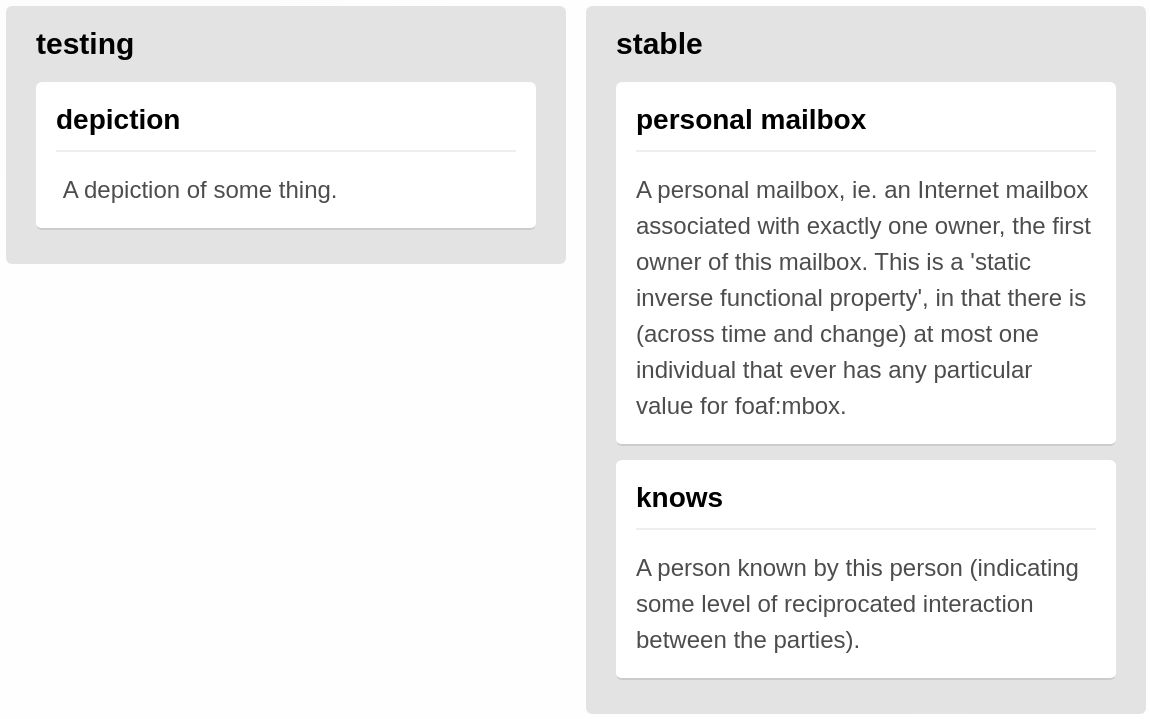
\includegraphics[width=125mm]{img/react-trello-example.png}
	\caption[Default react-trello Board]{Default react-trello board visualizing the data from \autoref{lst:React-Trello-Minimal-Data}.}
	\label{fig:react-trello-example}
\end{figure}



\subsubsection{Bypassing Limitations}

Without any modifications, the default card element of react-trello (as shown above) is limited to a predefined amount of elements it can possibly depict on its surface. However, react-trello allows developers to use their own card component. This provides two fundamental benefits: (1) Developers have no boundaries regarding card styling and positioning of elements, and (2) every value of a key that is specified within the card object of the data model can be depicted on a card. For example, the key \texttt{modified} at line 17 in previous \autoref{lst:React-Trello-Minimal-Data} can be used as a visual element within a custom card component (see line 8 in \autoref{lst:react-trello-customCardsDefinition}).

The following two code samples demonstrate the specification for a custom card component (\autoref{lst:react-trello-customCardsDefinition}) and the necessary changes within the react-trello component (\autoref{lst:react-trello-customCards}). Note that the properties used in \autoref{lst:react-trello-customCardsDefinition} (e.g., \texttt{modified} in lines 2 and 8) need to match exactly the key names defined within the data model in \autoref{lst:React-Trello-Minimal-Data}


\begin{spacing}{0.9}
    \lstset{language=JavaScript}
    \begin{lstlisting}[
    label={lst:react-trello-customCardsDefinition},
    xleftmargin=13em, % this needs to be manually adjusted to center the frame
    xrightmargin=-13em, % this needs to be manually adjusted to center the frame
    caption={[Example of a Custom Card Component]Example of a custom card component.}]
/* Custom Card Function at CustomCard/CustomCard.js */
export default ({title, description, modified, id}) => {
  return (
    <div>
      <h1>{title}</h1>
      <p>{description}</p>
      <hr />
      <p><small>{modified}</small></p>
      <p><a href={id}>{id}</a><p>
    </div>
  )
};
    \end{lstlisting}
\end{spacing}

\noindent In order to use the prior defined custom card components the main react-trello component requires the attribute \texttt{customCardLayout} (line 6) and the child element \texttt{<CustomCard \textbackslash>} (line 7) to be set.

\begin{spacing}{0.9}
    \lstset{language=JavaScript}
    \begin{lstlisting}[
    label={lst:react-trello-customCards},
    xleftmargin=16em, % this needs to be manually adjusted to center the frame
    xrightmargin=-16em, % this needs to be manually adjusted to center the frame
    caption={[Usage of Custom Cards]Usage of custom cards in react-trello.}]
/* Main React Component */
import Board from 'react-trello';
import CustomCard from './CustomCard/CustomCard';
/* ... */
return(
  <Board data={data} customCardLayout>
    <CustomCard />
  </Board>
);
    \end{lstlisting}
\end{spacing}

\noindent At this stage, the former code samples describe the core building blocks in order to create and display a board with an arbitrary amount of columns and cards. Although react-trello’s data model does not support swimlanes, this limitation can be bypassed by loading multiple instances of the board component, each containing a different data chunk, as depicted in lines 6 and 7 in \autoref{lst:react-trello-multipleBoards}. This means that, conceptually, each react-trello board can be considered as a swimlane. To obfuscate the semantic mapping from board to swimlane, the import statement might by renamed from \texttt{Board} to \texttt{Lane} (see lines 2, 6, and 7).

\begin{spacing}{0.9}
    \lstset{language=JavaScript}
    \begin{lstlisting}[
    label={lst:react-trello-multipleBoards},
    xleftmargin=21em, % this needs to be manually adjusted to center the frame
    xrightmargin=-21em, % this needs to be manually adjusted to center the frame
    caption={[Example of Multiple Swimlanes]Example of multiple swimlanes.}]
/* Main React Component */
import Lane from 'react-trello';
/* ... */
return(
  <div id="board-container">
    <Lane data={data1} />
    <Lane data={data2} />
  </div>
);
    \end{lstlisting}
\end{spacing}


\noindent Additionally, the existing data model needs to be adjusted to include swimlanes. \autoref{lst:react-trello-multipleLanesJSON} specifies a \acrshort*{JSON} template that acts as a superset of react-trellos’s data model. The benefit of this design is that it is (a) able to manage swimlanes, and (b) when destructuring the object by swimlanes, the resulting object satisfies the requested target data model by react-trello (lines 5 to 24 and 28 to 52). The adjusted model below consists of two swimlanes (lines 2 and 26) and two columns (lines 7f., 19f., and 30f., 42f. resp). While the first lane contains one card (line 9ff.) which is located in the column labeled \texttt{[Column Title\#1]} (line 7f.), the second column within this lane has no card (line 21). The second lane contains two cards, each of which are grouped in a different column (lines 32ff. and 44ff.)

\begin{spacing}{0.9}
    \lstset{language=JavaScript}
    \begin{lstlisting}[
    label={lst:react-trello-multipleLanesJSON},
    xleftmargin=13em, % this needs to be manually adjusted to center the frame
    xrightmargin=-13em, % this needs to be manually adjusted to center the frame
    caption={[Template Specification for Multiple Swimlanes]Template specification for multiple swimlanes within the data model.}]
{
  "[SWIMLANE IRI#1]": { // swimlane identifier
    "title": "[Swimlane Title#1]",
    // start of the react-trello format
    "lanes": [ // "columns" within the current swimlane
      {
        "title": "[Column Title#1]",
        "id": "[Column IRI#1]",
        "cards": [
          {
            "title": "[Card Title#1]",
            "id": "[Card IRI#1]",
            "description": "...",
            "modified": "[ISO 8601 Timestamp]"
          }
        ]
      },
      {
        "title": "[Column Title#2]",
        "id": "[Column IRI#2]",
        "cards": []
      }
    ]
    // end of the react-trello format
  },
  "[SWIMLANE IRI#2]": {
    "title": "[Swimlane Title#2]",
    "lanes": [
      {
        "title": "[Column Title#1]",
        "id": "[Column IRI#1]",
        "cards": [
          {
            "title": "[Card Title#2]",
            "id": "[Card IRI#2]",
            "description": "...",
            "modified": "[ISO 8601 Timestamp]"
          }
        ]
      },
      {
        "title": "[Column Title#2]",
        "id": "[Column IRI#2]",
        "cards": [
          {
            "title": "[Card Title#3]",
            "id": "[Card IRI#3]",
            "description": "...",
            "modified": "[ISO 8601 Timestamp]"
          }
        ]
      }
    ]
  }
}
    \end{lstlisting}
\end{spacing}


\subsection{RMB Specification}\label{ssec:BoardAnatomy}

This subsection provides the specification for the \acrshort*{UI} components that are used by the Resource Management Board. As outlined in the non-functional requirement \tracknshrink{NFR}\textsubscript{2}, eccenca has elaborated a style guide for its visual components based on Material Design Lite (\tracknshrink{MDL}).\footnote{\tracknshrink{MDL} is a \acrshort*{UI} component library by Google. GitHub: \url{https://github.com/google/material-design-lite}.} The corresponding specifications are publicly available\footnote{eccenca \acrshort*{UI} Repository: \url{https://github.com/eccenca/ecc-gui-elements}.} and will be referenced throughout this section.


\subsubsection{Cards}

To conform to eccenca’s visual appearance and to allow an arbitrary amount of elements to be depicted on a card’s surface, eccenca’s card component\footnote{Card specs. \url{https://github.com/eccenca/ecc-gui-elements\#card}.} replaces react-trello’s default card component.

\autoref{fig:CardTemplateMDL} illustrates the design and positioning specification for the card component. \autoref{fig:CardTemplateMDL}~(A) showcases all defined card component resources that a user may specify within the board configuration. However, the only mandatory elements on a card are its title and its resource identifier, as depicted by \autoref{fig:CardTemplateMDL} (B). This means, if an optional element (e.g., the description) is not defined within a resource, the card does not reserve a blank area. In other words, the card’s height matches its content. Moreover, the card specification contains different sections. For this work the following sections are relevant: \autoref{fig:CardTemplateMDL} (1) defines the \texttt{<CardTitle>}, (2) \texttt{<CardContent>} is used for the descriptive text, (3) and (4) use the element \texttt{<CardActions>}, since by design it creates a horizontal divider, and is set in a smaller font size.



\begin{figure}[H]
    \libertineLF
	\centering \begin{tikzpicture}
	\node[anchor=south west,inner sep=0] (image) at (0,0,0) {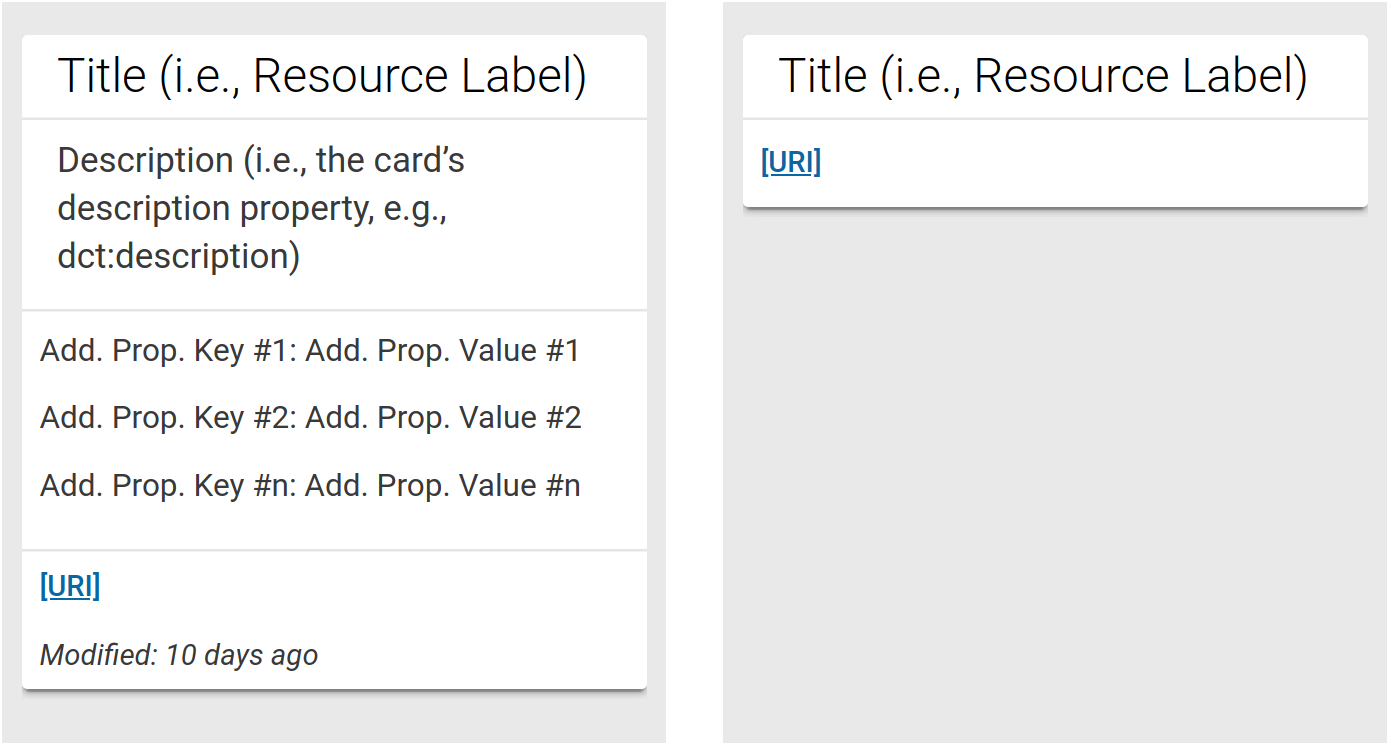
\includegraphics[width=114mm]{img/CardTemplateCompare.png}};
	\begin{scope}[x={(image.south east)},y={(image.north west)}]
% 	% next four lines will help you to locate the point needed by forming a grid. comment these four lines in the final picture.↓
% 		\draw[help lines,xstep=.1,ystep=.1] (0,0) grid (1,1);
% 		\draw[help lines,xstep=.05,ystep=.05] (0,0) grid (1,1);
% 		\foreach \x in {0,1,...,9} { \node [anchor=north] at (\x/10,0) {0.\x}; }
% 		\foreach \y in {0,1,...,9} { \node [anchor=east] at (0,\y/10) {0.\y};}
% 	% upto here↑
	

	\draw (0.210,1.050) node[anchor=west] {(A)};
	\draw (0.725,1.050) node[anchor=west] {(B)};
	\draw (-0.050,0.900) node[anchor=west] {(1)};
	\draw [fill=darkgray] (0.015,0.900) circle (.5ex);
	\draw (-0.050,0.700) node[anchor=west] {(2)};
	\draw [fill=darkgray] (0.015,0.700) circle (.5ex);
	\draw (-0.050,0.445) node[anchor=west] {(3)};
	\draw [fill=darkgray] (0.015,0.445) circle (.5ex);
	\draw (-0.050,0.157) node[anchor=west] {(4)};
	\draw [fill=darkgray] (0.015,0.157) circle (.5ex);
	
	\end{scope}
	\end{tikzpicture}
	\caption[Card Style \& Positioning Specification]{Card style and positioning specification.}
	\label{fig:CardTemplateMDL}
	\libertineOsF
\end{figure}

\paragraph{\tracknshrink{SHACLINE}} Whenever a user clicks a card, a modal window\footnote{A modal window is \textit{“[\textellipsis{}] a window overlaid on either the primary window or another dialog window. Windows under a modal dialog are inert. That is, users cannot interact with content outside an active dialog window.” \parencite{W3CDialog2015}}} appears and provides more information about the clicked resource. More specifically, the board requires an event handler that listens to card on-click events. This means, that the handler should receive the card’s resource identifier and the corresponding card’s graph. These two information are provided to eccenca’s \tracknshrink{SHACLINE} component, which creates a \acrshort*{SHACL}-defined document-like view on the provided resource and allows the user to manipulate data safely. The \tracknshrink{SHACLINE} component should be embedded within the modal window.



\subsubsection{Board Overview}

\autoref{fig:BoardTemplateMDL} specifies the structural layout of the Resource Management Board using the adjust swimlane model and eccenca \acrshort*{UI} elements. Foremost, \autoref{fig:BoardTemplateMDL} (1) uses the \texttt{<SelectBox>} element\footnote{SelectBox specs. \url{https://github.com/eccenca/ecc-gui-elements\#selectbox}.} allowing users to view all boards by their title. Moreover, the initial state of the application only displays the \texttt{<SelectBox>} element waiting for the user to select a board. After a board got selected, the remaining elements (2) to (6) appear below the selection box. Specifically, the elements (2) and (3) display the board’s title and description. The placeholder (4) should provide information or warnings about the state of the board (using the \texttt{<InfoBox>}\footnote{InfoBox specs. \url{https://github.com/eccenca/ecc-gui-elements\#alert-error-info-success-and-warning}.} element). Element (5) provides the label of the current swimlane. If swimlanes are not defined, this element does not appear. Lastly, the swimlane container (6) iterates over all swimlane objects defined in the data (at least once). It groups cards and columns in the way as specified before.

\begin{figure}[H]
    \libertineLF
	\centering \begin{tikzpicture}
	\node[anchor=south west,inner sep=0] (image) at (0,0,0) {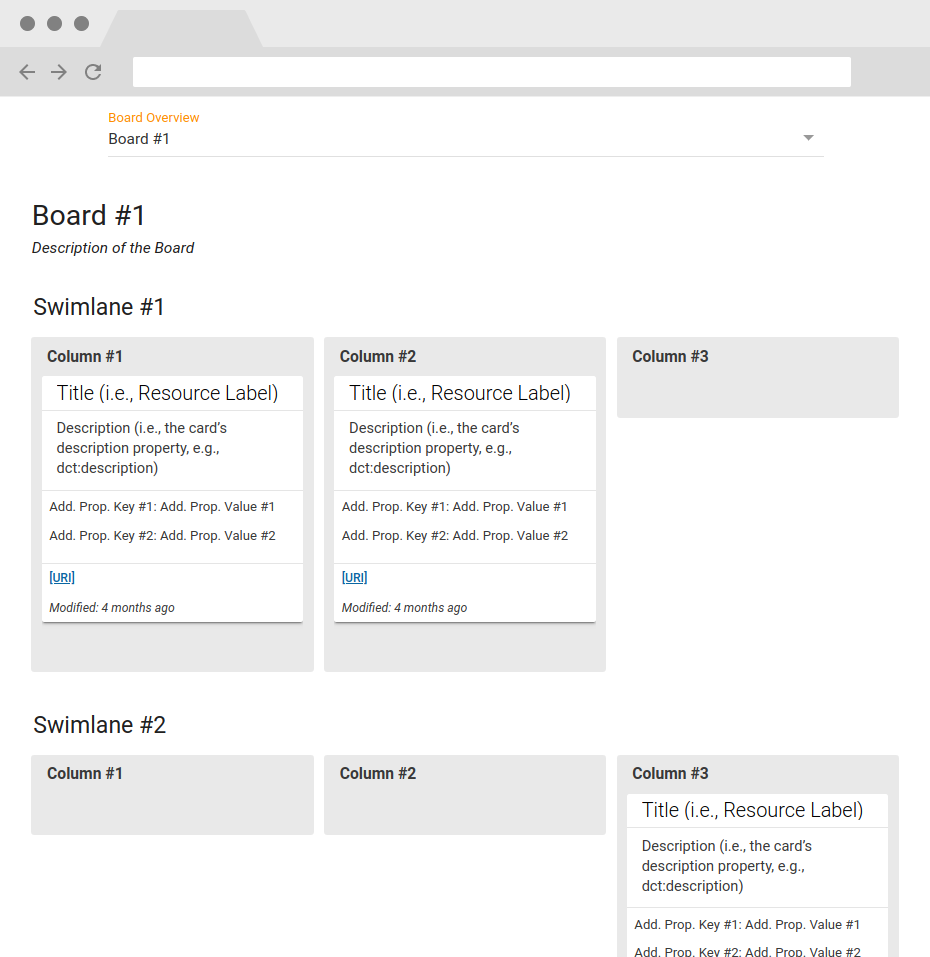
\includegraphics[width=\linewidth]{img/RMB-Browser-Specs.png}};
	\begin{scope}[x={(image.south east)},y={(image.north west)}]
% 	% next four lines will help you to locate the point needed by forming a grid. comment these four lines in the final picture.↓
% 		\draw[help lines,xstep=.1,ystep=.1] (0,0) grid (1,1);
% 		\draw[help lines,xstep=.05,ystep=.05] (0,0) grid (1,1);
% 		\foreach \x in {0,1,...,9} { \node [anchor=north] at (\x/10,0) {0.\x}; }
% 		\foreach \y in {0,1,...,9} { \node [anchor=east] at (0,\y/10) {0.\y};}
% 	% upto here↑
	

	\draw (-0.037,0.856) node[anchor=west] {(1)};
	\draw [fill=darkgray] (0.015,0.856) circle (.5ex);
	\draw (-0.037,0.775) node[anchor=west] {(2)};
	\draw [fill=darkgray] (0.015,0.775) circle (.5ex);
	\draw (-0.037,0.742) node[anchor=west] {(3)};
	\draw [fill=darkgray] (0.015,0.742) circle (.5ex);
	\draw (-0.037,0.712) node[anchor=west] {(4)};
	\draw [fill=darkgray] (0.015,0.712) circle (.5ex);
	\draw (-0.037,0.680) node[anchor=west] {(5)};
	\draw [fill=darkgray] (0.015,0.680) circle (.5ex);
	\draw (-0.037,0.640) node[anchor=west] {(6)};
	\draw [fill=darkgray] (0.015,0.640) circle (.5ex);
	
	\end{scope}
	\end{tikzpicture}
	\caption[Material Design Lite Mockup of the RMB]{Layout Specification for the RMB using react-trello and \tracknshrink{MDL} cards.}
	\label{fig:BoardTemplateMDL}
	\libertineOsF
\end{figure}


